\pagenumbering{arabic}

\section{示例}

\subsection{插入图片}
如图\ref{fig:top_realmeaning}所示\\
\begin{figure}[thbp!]
\centering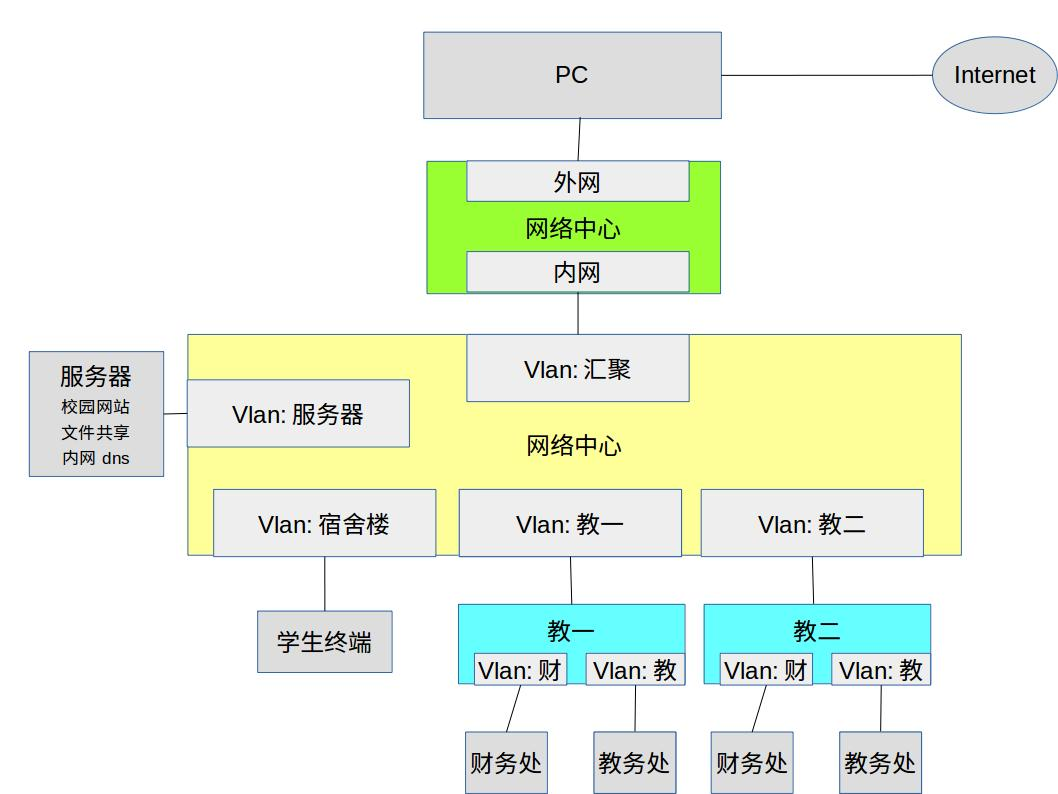
\includegraphics[width=0.9\linewidth]{figure/top_realmeaning.jpg}
\caption{ 模拟场景}
\label{fig:top_realmeaning}
\end{figure}

\subsection{插入代码}
\begin{lstlisting}[language=matlab]
  a=a;
  b=b;
  c=xxx;
\end{lstlisting}

\subsection{插入表格}
\begin{tabular}{cc}%一个c表示有一列,格式为居中显示(center)
(1,1)&(1,2)\\%第一行第一列和第二列  中间用&连接
(2,1)&(2,2)\\%第二行第一列和第二列  中间用&连接
\end{tabular}

\subsection{关于缩进}
\indent \textbf{xxxx}\\
\noindent xxxx

\subsection{list}
\begin{enumerate}
	\item A
	\item B
	\item C
\end{enumerate}

